\chapter{Re\c{t}ele neuronale convolu\c{t}ionale}

Re\c{t}elele neuronale convolu\c{t}ionale  sunt foarte similare cu re\c{t}elele neuronale obi\c{s}nuite din capitolul anterior, ele sunt formate din neuroni care \^{i}nva\c{t}\u{a} ponderi \c{s}i bias-uri care s\u{a} \^{i}ndeplineasc\u{a} o anumit\u{a} sarcin\u{a}. Fiecare neuron prime\c{s}te date de intrare de la neuronii de pe nivelul inferior lor, efectuaz\u{a} o opera\c{t}ie de multiplicare \^{i}ntre ponderi \c{s}i datele de intrare, adun\u{a} bias-ul la rezultatul ob\c{t}inut \^{i}n urma multiplic\u{a}rii, iar dup\u{a}, de cele mai multe ori aplic\u{a} o func\c{t}ie de activare. La final dup\u{a} ultimul nivel aplic\u{a} o func\c{t}ie de cost care s\u{a} determine c\^{a}t de aproape este re\c{t}eaua neuronal\u{a} de adev\u{a}r \c{s}i dup\u{a} se aplic\u{a} propagarea \^{i}napoi pentru a actualiza ponderile \c{s}i bias-ruile de pe fiecare nivel astfel \^{i}nc\^{a}t la urmatorul pas de \^{i}nv\u{a}\c{t}are a re\c{t}elei neuroanle aceasta s\u{a} ob\c{t}in\u{a} un rezultat mai mic de la func\c{t}ia de cost.

La prima vedere re\c{t}elele neuronale convolu\c{t}ionale seaman\u{a} foarte mult cu re\c{t}elele neuronale obi\c{s}nuite, un lucru adev\u{a}rat, \^{i}ns\u{a} exista unele diferen\c{t}e \^{i}ntre ele. Re\c{t}elele neuronale convolu\c{t}ionale pleac\u{a} de la prezum\c{t}ia c\u{a} datele de intrare de pe primul nivel sunt imagini, fa\c{t}\u{a} de re\c{t}elele neuronale obi\c{s}nuite, unde datele de intrare de pe primul nivel sunt ni\c{s}te vectori. Din aceast\u{a} cauz\u{a} re\c{t}elele neuronale convolu\c{t}ionale se pot folosii de unele propiet\u{a}\c{t}i ale imaginilor, asfel \^{i}nc\^{a}t acestea s\u{a} fiu mai eficiente in sarcini ce implic\u{a} imaginile \c{s}i mai u\c{s}or de antrenat deoarece au nevoie de mai pu\c{t}ini parametrii dec\^{a}t ar avea nevoie o re\c{t}ea nuronal\u{a} obi\c{s}nuit\u{a} \^{i}n \^{i}ndeplinirea aceleia\c{s}i sarcini.

\section{Arhitectura unei re\c{t}ele neuronale convolu\c{t}ionale}

Cum am v\u{a}zut in capitolul anterior, re\c{t}elele neuronale obi\c{s}nuite primesc ca date de intrare un  vector pe care \^{i}l trec prin mai multe nivele de neuroni, unde fiecare neuron de pe un nivel este conectat cu to\c{t}i neuronii de pe nivelul urm\u{a}tor \c{s}i cu to\c{t}i neuronii de pe nivelul inferior lui, \^{i}ns\u{a} nu este conectat cu neuronii de pe acela\c{s} nivel cu el. 

\par

Faptul c\u{a} re\c{t}elele neuronale convolu\c{t}ionale sunt concepute special pentru sarcini ce implic\u{a} imagini \c{s}i c\u{a} datele de intrare  au trei dimensiuni ( l\u{a}\c{t}ime, \^{i}n\u{a}l\c{t}ime \c{s}i ad\^{a}ncime ),  fa\c{t}\u{a} de re\c{t}elele neuronale obi\c{s}nuite unde datele de intrare au o singur\u{a} dimensiune, neuronii de pe nivele trebuiesc rearanja\c{t}i astfel \^{i}nc\^{a}t s\u{a} \^{i}ndeplineasc\u{a} c\^{a}t mai bine sarcina pe care o au de f\u{a}cut \c{s}i s\u{a} se folosesc\u{a} c\^{a}t mai bine de propriet\u{a}\c{t}ile pe care le au imaginile. Din aceast\u{a} cauz\u{a} neuronii de pe un nivel la o re\c{t}ea neuronal\u{a} convolu\c{t}ional\u{a} sunt aranja\c{t}i pe trei dimensiuni ( l\u{a}\c{t}ime, \^{i}n\u{a}l\c{t}ime \c{s}i ad\^{a}ncime ), \^{i}n compara\c{t}ie cu re\c{t}elele neuronale obi\c{s}nuite unde neuronii erau aranja\c{t}i pe o singura dimensiune, cu acest timp de aranjament neuronii vor creea ponderi ce vor pune \^{i}n eviden\c{t}\u{a} anumite caracteristici ale unei imagine, caracteristici ce vor asigura o mai bun\u{a} performan\c{t}\u{a} a re\c{t}elei. Astfel c\u{a} un nivel dintr-o re\c{t}ea neuronal\u{a} convolu\c{t}ional\u{a} prime\c{s}te un volum de date cu trei dimensiuni \c{s}i produce un volum de date tot cu trei dimensiuni, volum de date care va fi dat mai departe la nivelul urm\u{a}tor lui.

\par 

\begin{center}
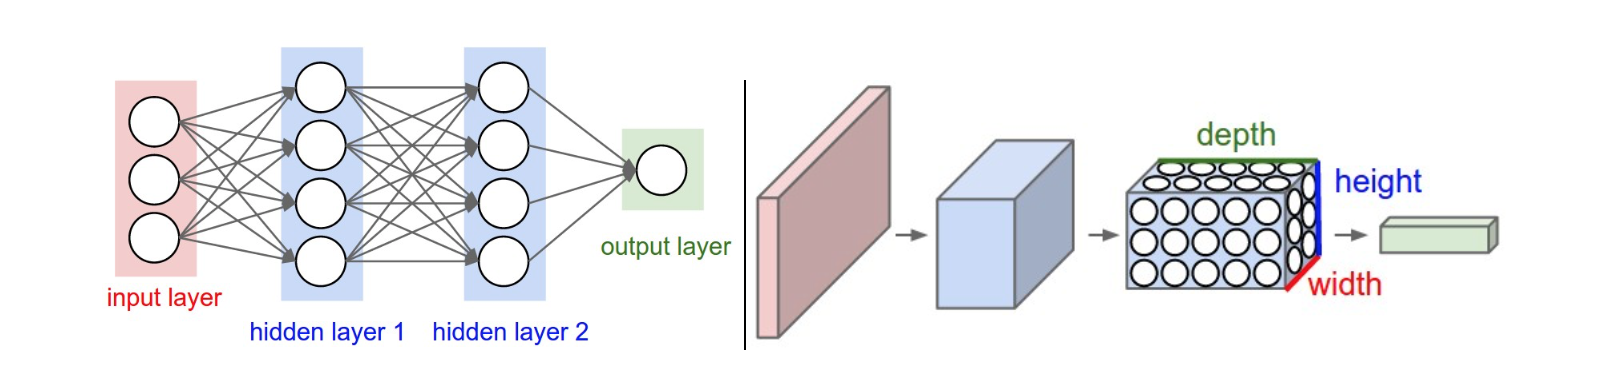
\includegraphics[width=450]{nn_cnn.png}
\end{center}

Imaginea de mai sus se arat\u{a} diferen\c{t}a \^{i}ntre modul de aranjare a neuronilor pe o re\c{t}ea neuronal\u{a} obi\c{s}nuit\u{a} \c{s}i o re\c{t}ea neuronal\u{a} convolu\c{t}ional\u{a}.

\^{I}n re\c{t}elele neuronale convolu\c{t}ionale exit\u{a} trei tipuri de nivele, fa\c{t}\u{a} de re\c{t}elele neuronale obi\c{s}nuite unde exist\u{a} doar un singur tip, aceste nivele dintr-o re\c{t}ea neuronal\u{a} se numesc: nivelul convolu\c{t}ional, nivelul de pool \c{s}i nivelul conectat complet.

\subsection{Nivelul convolu\c{t}ional}

Nivelul convolu\c{t}ional este cel mai important nivel din cele trei \c{s}i cel care influen\c{t}eaz\u{a} cel mai mult deciziile re\c{t}elei neuronale. Acest nivel, ca \c{s}i nivelele din re\c{t}elele neuronale are dou\u{a} tipuri de paramterii, ponderile \c{s}i bias-urile, ins\u{a} \^{i}nt\u{a}ririle sunt organizate pe trei dimensiuni cum am discutat mai sus, astfel \^{i}nc\^{a}t acestea s\u{a} devin\u{a} ni\c{s}te filtre care \^{i}n urma aplic\u{a}rii lor asupra datelor de intrare s\u{a} scoat\u{a} \^{i}n eviden\c{t}\u{a} unele detalii descriminatorii care s\u{a} ajute la \^{i}ndeplinirea sarcinii, \^{i}ns\u{a} bias-urile sunt la fel ca la neuronii din re\c{t}elele neuronale obi\c{s}nuite. 

\par

De cele mai multe ori ponderile sunt mici \^{i}n \^{i}n\u{a}l\c{t}ime \c{s}i l\u{a}\c{t}ime dar sunt foarte mari in ad\^{a}ncime. [3x3x512] este un exemplu de dimensiune a unei ponderi, unde \^{i}n\u{a}\c{t}imea \c{s}i l\u{a}\c{t}imea au dimensiune 3, iar ad\^{a}ncimea are dimensiunea 512, motivul pentru care ad\^{a}ncimea este a\c{s}a de mare, iar \^{i}n\u{a}l\c{t}imea \c{s}i l\u{a}\c{t}imea au dimensiuni a\c{s}a de mici  este pentru c\u{a} \^{i}n acest mod se pot construii mai multe filtre pe o por\c{t}iune mai mic\u{a} din datele de intrare \c{s}i, cum vom vedea in capitolele urm\u{a}toare, acest lucru faciliteaz\u{a} \^{i}n mod pozitiv acurate\c{t}ea re\c{t}elei neuronale.

\par

Nivelul convolu\c{t}ional gliseaz\u{a} o fereastr\u{a} de dimensiunea ponderilor de-a lungul \c{s}i de-a latul datelor de intrare pornind de la col\c{t}ul de sus stanga a datelor de intrare \c{s}i face o \^{i}nmul\c{t}ire \^{i}ntre  datele de intrare aflate \^{i}n fereastr\u{a} \c{s}i cu ponderile \c{s}i  dup\u{a} la rezultat este adunat bias-ul. Acest proces este repetat p\^{a}n\u{a} c\^{a}nd fereastra ajunge in col\c{t}ul de jos dreapta a datelor de intrare. \^{I}n urma acestui proces va rezulta un volum de date bidimensional, dar acest proces este repetat pentru fiecare pondere asftel c\u{a} la final vom avea un volum de date tridimensional. Cum am mai spus \c{s}i mai sus ponderile \^{i}ntr-o re\c{t}ea neuronal\u{a} convolu\c{t}ional\u{a} sunt ni\c{s}te filtre care scot \^{i}n eviden\c{t}\u{a} anumte aspecte ale datelor de intrare, cum ar fi marginea unui obiect aflat \^{i}n imagine, o anumit\u{a} structur\u{a} care este caractersitic\u{a} unei anumite categorii de obiecte sau un \c{s}ablon.

\par

Pentru a se \^{i}n\c{t}elege mai bine cum func\c{t}ioneaz\u{a} nivelul convolu\c{t}ional s\u{a} presupunem c\u{a} avem o imagine de dimesniune [28x28x3] iar o pondere are dimensiunea [5x5x3], a se observa faptul c\u{a} at\^{a}t  ponderea c\^{a}t \c{s}i imaginea au aceea\c{s}i ad\^{a}ncime, respectiv 3, tot timpul ad\^{a}ncimea ponderilor trebuie s\u{a} fie identic\u{a} cu cea a datelor de intrare pentru c\u{a} \^{i}n caz contrar nu s-ar putea face \^{i}nmul\c{t}irea \^{i}ntre datele de intrare \c{s}i ponderi, \^{i}ns\u{a} \^{i}n\u{a}l\c{t}imea \c{s}i l\u{a}\c{t}imea ponderilor trebuie s\u{a} fie neap\u{a}rat mai mici dec\^{a}t a datelor de intrare astfel, nu s-ar putea face glisarea. Dimensiunea ponderilor \^{i}n \^{i}n\u{a}l\c{t}ime \c{s}i l\u{a}\c{t}ime este setat\u{a} manual, fiind un parametru important de setat \^{i}ntr-o re\c{t}ea neuronal\u{a} convolu\c{t}ional\u{a}. 

\begin{center}
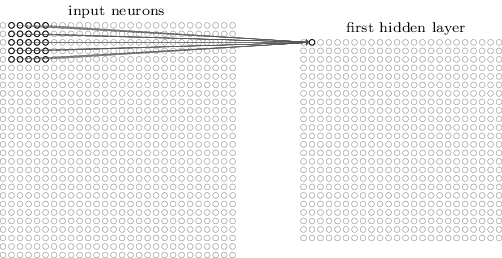
\includegraphics[width=300]{conv.png}
\end{center}

Cum se observ\u{a} \c{s}i \^{i}n imaginea de mai sus \^{i}n loc s\u{a} mai lu\u{a}m fiecare valoare a unui pixel separat \c{s}i s\u{a} o introducem \^{i}ntr-un neuron de pe un nivel intermediar ( hidden layer ) ca dat\u{a} de intrare putem s\u{a} grup\u{a}m pixelii in blocuri de pixeli \c{s}i s\u{a} \^{i}i trimitem grupa\c{t}i la un neuron de pe nivelul intermediar. \^{I}n cazul nostru vom face glisarea pe un grup de pixeli de dimensiunea [5x5x3] care va fi \^{i}nmul\c{t}it cu ponderile noastre de dimensiune [5x5x3], \^{i}n urma rezultatului vom ob\c{t}ine o singur\u{a} valoare la care vom aduna bias-ul. Dac\u{a} se repet\u{a} procedeul  \c{s}i ne mi\c{s}c\u{a}m cu un pixel la dreapta, sau in jos pentru fiecare bloc de pixeli pe care vrem s\u{a} \^{i}l extragem, atunci ca rezultat vom avea [24x24x1] de valori. Acum s\u{a} presupunem c\u{a} avem 32 de astfel de ponderi pe acest nivel \c{s}i reptet\u{a}m procedeul pentru fiecare, atunci, ca rezultat final vom avea [24x24x32] de valori, valori care vor fi trimise mai departe c\u{a}tre urm\u{a}torul nivel. Un mare beneficiu al acestui mod de a grupa valorile \^{i}n blocuri de date mai mici, peste care s\u{a} efectu\u{a}m opera\c{t}ia de \^{i}nmul\c{t}ire \c{s}i de adunare este c\u{a} se reduce semnificativ num\u{a}rul de valori la o  ponder\u{a} de care am fi avut nevoie dac\u{a} am fi f\u{a}cut acela\c{s} lucru pentru toate datele dintr-o dat\u{a}, cum se face \^{i}ntr-o re\c{t}ea neuronal\u{a} obi\c{s}nuit\u{a}, spre exemplu \^{i}n cazul exemplificat mai sus avem nevoie doar de 5 x 5 x 3 = 75 de valori pentru o ponder\u{a}, \^{i}n cazul unei re\c{t}ele neuronale obi\c{s}nuite am fi avut nevoie de 28 x 28 x 3 = 2352 de valori pentru o ponder\u{a}. Prin reducerea numarului de valori de care avem nevoie pentru o ponder\u{a} vom cre\c{s}te viteza de \^{i}nv\u{a}\c{t}are a re\c{t}elei neuronale \c{s}i vom putea cre\c{s}te complexitatea acesteia.

\par

Mai sus am discutat despre cum nivelul convolu\c{t}ional transform\u{a} un volum de date tridimensional \^{i}ntr-un alt volum de date tridimensional \c{s}i cum \^{i}l calculeaz\u{a} pe acesta, \^{i}ns\u{a} nu am discutat cum se calculeaz\u{a} dimensiunea volumului de date tridimensional rezultat \^{i}n urma aplicarii nivelului convolu\c{t}ional peste  datele de intrare. Sunt trei parametrii care controleaz\u{a} m\u{a}rimea datelor de ie\c{s}ire dintr-un nivel convolu\c{t}ional, acestea sunt: ad\^{a}ncimea, pasul de mi\c{s}care a ferestrei c\^{a}nd se face glisarea ei peste volumul de date \c{s}i padding-ul. Ad\^{a}ncimea corespunde numarului de ponderi pe care \^{i}l are respectivul nivel convolu\c{t}ional. Pasul este c\^{a}t de mult se mi\c{s}c\u{a} fereastra c\^{a}nd se face glisarea peste datele de intrare, dac\u{a} pasul este unu, atunci fereastra se va mi\c{s}ca la dreapta c\^{a}te un pixel, iar c\^{a}nd va ajunge la cap\u{a}t va cobor\^{i} un pixel \c{s}i va merge din noul la dreapta c\^{a}te un pixel p\^{a}n\u{a} la cap\u{a}t, acest procedeu repet\^{a}ndu-se p\^{a}n\u{a} c\^{a}nd fereastra va ajunge \^{i}n col\c{t}ul de jos din dreapta. Dac\u{a} pasul este doi, atunci fereastra se va mi\c{s}ca doi pixeli la dreapta \c{s}i \^{i}n jos, \^{i}ns\u{a} acest lucru va produce mai pu\c{t}ine date de ie\c{s}ire dec\^{a}t dac\u{a} pasul era unu. Padding-ul presupune numarul de r\^{a}nduri cu valoare zero pe care le punem \^{i}n jurul datelor de intrare astfel \^{i}nc\^{a}t s\u{a} putem controla dimensiunea datelor de ie\c{s}ire. Spre exemplu cum aveam mai sus o imagine de dimesniune [28x28x3] \c{s}i ponderi de dimensiunea [5x5x3] \c{s}i un pas de unu aveam ca rezultat un volum de date de dimensiunea [24x24x1] pentru o ponder\u{a}, \^{i}ns\u{a} dac\u{a} ad\u{a}ug\u{a}m un padding de doi in jurul imaginii, atunci vom avea un volum de date de dimensiunea [32x32x3], deoarece padding-ul de doi s-a adugat jos, sus, la st\^{a}nga c\^{a}t \c{s}i la dreapta imaginii, iar \^{i}n urma aplic\u{a}rii nivelului convolu\c{t}ional peste noul set de date vom avea un rezultat de dimensiunea [28x28x1]. Se observ\u{a} faptul c\u{a} noul rezultat are aceea\c{s}i dimensiune, at\^{a}t pe \^{i}n\u{a}l\c{t}ime, c\^{a}t \c{s}i pe l\u{a}\c{t}ime ca dimensiunea datelor ini\c{t}iale \^{i}nainte de aplicarea padding-ului, acest lucru  de a pastra dimensiunea datelor de ie\c{s}ire egal cu cel al datelor de intrare pe \^{i}n\u{a}l\c{t}ime \c{s}i l\u{a}\c{t}ime este foarte des folosit \^{i}n practic\u{a}, deoarece prin acest fel se p\u{a}streaz\u{a} consisten\c{t}a datelor.

Putem s\u{a} exprim\u{a}m calculul volumului de ie\c{s}ire printr-o formul\u{a} foarte simpl\u{a} care arat\u{a} \^{i}n felul urm\u{a}tor:

$$ \frac{W - F + 2P }{S} + 1 $$

\^{I}n formula de mai sus, W este marimea volumui de date, F este m\u{a}rimea ferestrei prin care se face glisarea peste date, S este pasul de mi\c{s}care a ferestrei peste volumul de date, iar P este padding-ul care se adauga \^{i}n jurul volumului de date. Spre exemplu, dac\u{a} avem un volum de date de dimensiune 7x7 \c{s}i ponderi de dimensiunea 3x3 cu un pas de 1 \c{s}i un padding de 0 atunci vom avea un rezultat de dimensiunea 5x5, \^{i}ns\u{a} dac\u{a} cre\c{s}tem pasul la 2 atunci vom avea un rezultat de dimensiunea 3x3.

\par

La o mic\u{a} analiz\u{a} se poate observa faptul c\u{a} pasul glis\u{a}rii ferestrei are anumite constr\^{a}ngeri, spre exemplu dac\u{a} volumul de date are o dimesniune de [10x10], padding-ul este 0 iar m\u{a}rimea ferestrei este de [3x3], atunci ar fi imposibil s\u{a} folosim un pas de 2, deoarece

$$ \frac{W - F + 2P }{S} + 1 = \frac{10 - 3 + 0 }{2} + 1 = 4.5 $$

\c{s}i av\^{a}nd \^{i}n vedere faptul c\u{a} dimensiunea datelor de ie\c{s}ire trebuie s\u{a} fie un num\u{a}r \^{i}ntreg atunci ar fi imposibil s\u{a} folosim un pas de 2 \^{i}ntr-un astfel de caz. \^{I}n astfel de cazuri, dac\u{a} nu vrem s\u{a} schimb\u{a}m pasul, va trebuii s\u{a} adaug\u{a}m un padding \^{i}n jurul datelor de intrare astfel \^{i}nc\^{a}t s\u{a} ob\c{t}inem la final un num\u{a}r \^{i}ntreg ca dimensiune pentru volumul de date rezultat de c\u{a}tre nivelul convolu\c{t}ional, \^{i}n cazul nostru de mai sus dac\u{a} ad\u{a}ug\u{a}m un padding de 1, atunci vom avea  o dimensiune de [5x5] pentru volumul de date rezultat de c\u{a}tre nivelul convoli\c{t}ional.

\subsection{Niveulul de pool}

Nivelul de pooling se pune \^{i}ntre dou\u{a} nivele convolu\c{t}ionale pentru a se reduce cantitatea de informa\c{t}ie care se duce c\u{a}tre urm\u{a}torul nivel convolu\c{t}ional. Cel mai folosit tip de pooling este max-pooling care prime\c{s}te ca date de intrare valorile rezultate de la precedentul nivel convolu\c{t}ional \c{s}i le las\u{a} s\u{a} treac\u{a} doar pe cel cu valoarea cea mai mare c\u{a}tre urm\u{a}torul nivel convolu\c{t}ional ( vede\c{t}i imaginea de mai jos ), astfel c\u{a} acest nivel ne ajut\u{a} s\u{a} reducem cantitatea de date \c{s}i s\u{a} sc\u{a}p\u{a}m de datele nerelevante dintr-o re\c{t}ea convolu\c{t}ional\u{a}. 

\par

De cele mai multe ori nivelul max-pooling ia o fereastr\u{a} de dimensiune [2x2] \c{s}i o gliseaz\u{a} peste datele de intrare cu un pas de cu valoarea 2. La fiecare pas acest nivel ia valorile cuprinse \^{i}n fereastr\u{a} \c{s}i las\u{a} doar valoarea cea mai mare s\u{a} treac\u{a} mai departe, celelalte fiind eliminate. \^{I}n urma acestor opera\c{t}ii va fi redus\u{a} o catitate de 75\% din datele de intrare, spre exemplu dac\u{a} avem un volum de date de dimensiunea [32x32x32] \c{s}i aplic\u{a}m peste el un max-pool cu o fereastr\u{a} de dimensiunea [2x2] \c{s}i un pas de 2 atunci vom avea ca rezultat un volum de date de dimensiunea [16x16x32], de precizat faptul c\u{a} nivelul max-pool nu afecteaz\u{a} ad\^{a}ncimea datelor de intrare.

\begin{center}
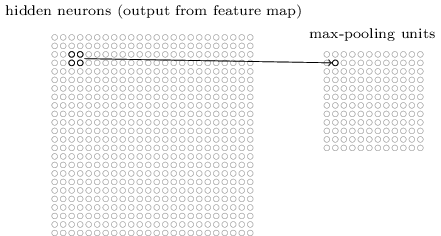
\includegraphics[width=300]{pool.png}
\end{center}

Cum se observ\u{a} \c{s}i \^{i}n imaginea de mai sus, nivelul de max-pooling prime\c{s}te patru valori de pe nivelul precedent \c{s}i las\u{a} o singur\u{a} valoarea s\u{a} treac\u{a} mai departe.

Un mare beneficiu pe care nivelul max-pool \^{i}l are asupra unei re\c{t}ele neuronale convolu\c{t}ionale este acela c\u{a} ne permite s\u{a} aplic\u{a}m nivele convolu\c{t}ionale mai mari peste date dup\u{a} ce am aplicat nivelul max-pool, acest lucru este posibil deoarece, cum am mai zis \c{s}i mai sus, nivelul max-pool ne scap\u{a} de o cantitate semnificativ\u{a} de date, prin urmare cantitate de date va fi mai mic\u{a} \c{s}i timpul de aplicare a unei \^{i}nt\u{a}riri va fi mai mic, prin urmare vom putea s\u{a} aplic\u{a}m mai multe \^{i}nt\u{a}riri la urm\u{a}torul nivel convolu\c{t}ional f\u{a}r\u{a} s\u{a} cre\c{s}tem timpul de calcul.

\subsection{Nivelul conectat complet}

Nivelul conectat complet este identic cu un nivel dintr-o re\c{t}ea neuronal\u{a} obi\c{s}nuit\u{a}, \^{i}n ideea c\u{a} fiecare neuron de pe nivelul inferior este conectat cu fiecare neuron de nivelul superior lui.

\par

Pentru a ad\u{a}uga un nivel conectat complet dup\u{a} un nivel convolu\c{t}ional, sau un nivel de pool, va trebuii s\u{a} redimension\u{a}m volumul de date trimidimensional care rezult\u{a} din astfel de nivele, pentru c\u{a}, nivelul conectat complet accept\u{a} ca date de intrare un volum de date unidimensional (vector). A\c{s}a c\u{a}, spre exemplu, atunci c\^{a}nd avem un volum de date rezultat dintr-un nivel convolu\c{t}ional de marimea, s\u{a} zicem, [7x7x512] va trebuii s\u{a} \^{i}l redimensionam la un vector cu 25088 de elemente, deoarece 7 x 7 x 512 = 25088, iar dup\u{a} aceea s\u{a} \^{i}numl\c{t}im datele redimensionate cu o \^{i}nt\u{a}rire de dimensiune, spre exemplu \^{i}n cazul pe care \^{i}l exemplific\u{a}m acum, [1024x25088] ,iar la rezultatul ob\c{t}inut \^{i}n urma \^{i}nmul\c{t}irii s\u{a} adun\u{a}m un bias, \^{i}n cazul nostru bias-ul  va avea 1024 de elemente.

\subsection{A\c{s}ezarea nivelelor}

Am v\u{a}zut p\^{a}n\u{a} acum c\u{a} re\c{t}elele neuronale convolu\c{t}ionale sun alc\u{a}tuite din trei tipuri de nivele (nivelul convolu\c{t}ional, nivelul de pool \c{s}i nivelul conectat complet). \^{I}n aceast\u{a} sec\c{t}iune vom discuta despre modalit\u{a}\c{t}ile de a a\c{s}eza aceste nivel \^{i}ntr-o re\c{t}ea neuronal\u{a} convolu\c{t}ional\u{a}.

\par

De cele mai multe ori o re\c{t}ea neuronal\u{a} convolu\c{t}ional\u{a} este alc\u{a}tuit\u{a} din mai multe nivele convolu\c{t}ionale, unde dup\u{a} fiecare nivel convolu\c{t}ional poate urma un nivel de pool, iar la final sunt ad\u{a}ugate unul sau mai multe nivele conectate complet unde ultimul nivel conectat complet va \^{i}ntoarce datele de ie\c{s}ire din re\c{t}eaua neuronal\u{a}. Cu alte cuvinte, de cele mai multe ori o re\c{t}ea neuronal\u{a} convolu\c{t}ional\u{a} respect\u{a} urm\u{a}torul tip de \c{s}ablon c\^{a}nd vine vorba de a\c{s}ezarea nivelelor :

\par

\text{Date de intrare} \longrightarrow [[\text{Nivel convolu\c{t}ional} \longrightarrow \text{ReLU}]*N \longrightarrow \\
\longrightarrow \text{Nivel pool ? } ] * M \longrightarrow [\text{Nivelul conectat complet} \longrightarrow \text{ReLU}] * K  \longrightarrow \\
\longrightarrow \text{Nivelul conectat complet} \longrightarrow \text{Date de ie\c{s}ire}

\^{I}n \c{s}ablonul de mai sus, stelu\c{t}a reprezint\u{a} de c\^{a}te ori se repet\u{a} secven\c{t}a de nivele din parantezele p\u{a}trate, iar N, M \c{s}i K reprezint\u{a} num\u{a}rul de repeti\c{t}ii, unde fiecarea valoare trebuie s\u{a} fie mai mare sau egal\u{a} cu zero. Am notat cu semnul \^{i}ntreb\u{a}rii nivelul pool doarece acesta poate ap\u{a}rea sau nu dup\u{a} nivelul convolu\c{t}ional.

\par

Un exemplu de astfle de re\c{t}ea neuronal\u{a} care s\u{a} respecte \c{s}ablonul de mai sus ar fi urm\u{a}toarea:

\text{Date de intrare} \longrightarrow \text{Nivel convolu\c{t}ional 1} \longrightarrow \text{ReLU} \longrightarrow \text{Nivel pool 1} \longrightarrow \\ 
\longrightarrow \text{Nivel convolu\c{t}ional 2} \longrightarrow \text{ReLU} \longrightarrow \text{Nivel pool 2} \longrightarrow \\ 
\longrightarrow  \text{Nivelul conectat complet} \longrightarrow \text{Date de ie\c{s}ire}

\^{I}n exemplul dat mai sus, N are valoarea 1, M are valoarea 2, iar K are valoarea 0.

\section{Procesul de antrenare}

A\c{s}a cum am precizat mai sus, la re\c{t}elele neuronale obi\c{s}nuite, procesul de antrenare const\u{a} \^{i}n actualizarea ponderilor \c{s}i bias-urilor dintr-o re\c{t}ea neuronal\u{a} cu o anumit\u{a} valoare, calculat\u{a} pe baza gradientului calculat \c{s}i \^{i}nmul\c{t}it\u{a} cu o constant\u{a}, care se nume\c{s}te rata de antrenare.

C\^{a}nd am discutat despre procesul de antrenare la re\c{t}ele neuronale obi\c{s}nuite am descris metoda SGD, \^{i}ns\u{a} a\c{s}a cum am preciza, SGD nu este suficent de eficent \c{s}i exist\u{a} alte metode mai eficinete de antrenare a unei re\c{t}ele neuronale. Metoda pe care o vom descrie mai jos, \c{s}i pe care o vom folosi \^{i}n procesul de antrenare a re\c{t}elelor neuronale convolu\c{t}ionale pe care le vom construii pentru a reozolva problema noastr\u{a}, se nume\c{s}te Adam.

\subsection{Adam}

Adam este o metod\u{a} nou\u{a} folosit\u{a} pentru actualizarea paramtetrilor dintr-o re\c{t}ea neuronal\u{a} obi\c{s}nuit\u{a}. Numele s\u{a}u deriveaz\u{a} din cuvintele adaptive moment estimation \c{s}i a fost inventat\u{a} de Diederik P. Kingma de la Universitatea din Amsterdam \c{s}i de Jimmy Lei Ba de la Universitatea din Toronto. Metoda propus\u{a} de ace\c{s}tia are urmatoarea formul\u{a}:

$$ m = \beta_1 \cdot m + ( 1 - \beta_1 ) \cdot \delta x $$
$$ v = \beta_2 \cdot v + ( 1- \beta_2 ) \cdot \delta x^2 $$
$$ x = x - \zeta \cdot \frac{m}{\sqrt{v} + \epsilon } $$

\^{I}n formulele de mai sus $\beta_1, \beta_2 $ \c{s}i $ \epsilon $ sunt trei constante pentru care autorii sugereaz\u{a} urmatoarele valor, $\beta_1 = 0.9 $, $\beta_2 = 0.999 $ \c{s}i $ \epsilon = 1e^{-8} $, vom pastra aceste valori \^{i}n re\c{t}elele noastre convolu\c{t}ionale. Valorile m \c{s}i v sunt la inceput ini\c{t}ializate cu valoarea zero, aceste valori, confomr autorilor, au rolul de a corecta anumite erori atunci c\^{a}nd se actualizeaz\u{a} parametrii re\c{t}elei. Cu $\zeta$ am notat rata de \^{i}mv\u{a}\c{t}are a re\c{t}elei neuronale.

\section{Procesarea datelor}

\^{I}nainte ca datele s\u{a} intre \^{i}ntr-o re\c{t}ea neuronal\u{a}, acestea trebuiesc preprocesate, astfle \^{i}nc\^{a} re\c{t}elei neuronale s\u{a} \^{i}i fie mai u\c{s}or s\u{a} \^{i}nve\c{t}e. Cele mai folosite metode de preprocesare a datelor sunt centrarea la origine a datelor \c{s}i normalizarea. Exist\u{a} o gramad\u{a} de metode de procesare a datelor, \^{i}ns\u{a} acestea sunt aplicabile doar pentru anumite seturi de date, \^{i}n timp ce, cele do\u{a} men\c{t}ionate mai sus sunt generale pentru orice tip de date \c{s}i pentru orice tip de re\c{t}ea neuronal\u{a}.

Pentru a exemplifica cum functioneaz\u{a} cele doua metode, vom presupune c\u{a} avem un set de date bidimensional ce are graficul urmator.

\begin{center}
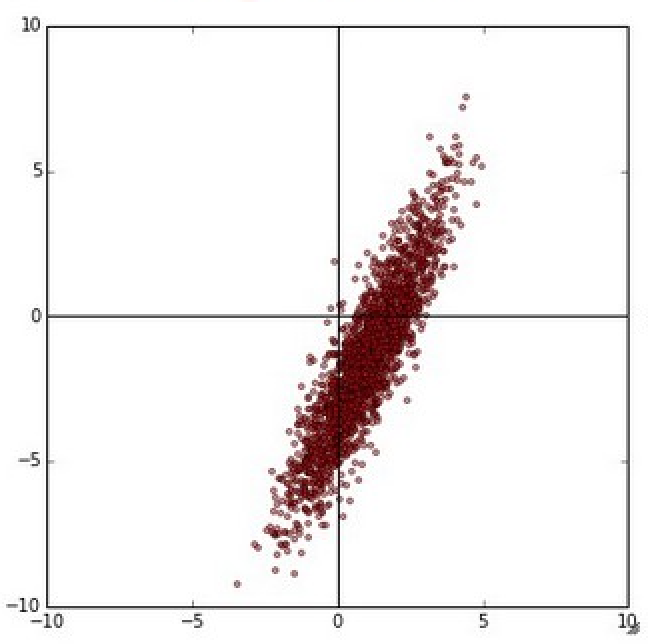
\includegraphics[width=200]{original.png}
\end{center}

Centrarea la origine a datelor, presupune c\u{a} pentru fiecare valorea s\u{a} sc\u{a}dem media valorilor din respectivul set de date.

            $$ X = X - \frac{1}{N}\sum_i^N X_i$$
            
Aceast\u{a} opera\c{t}ie va aduce centrul datelor la origine. \^{I}n cazul nostru de mai sus, dup\u{a} aplicarea opera\c{t}iei, graficul datelor va ar\u{a}ta \^{i}n felul urm\u{a}tor.

\begin{center}
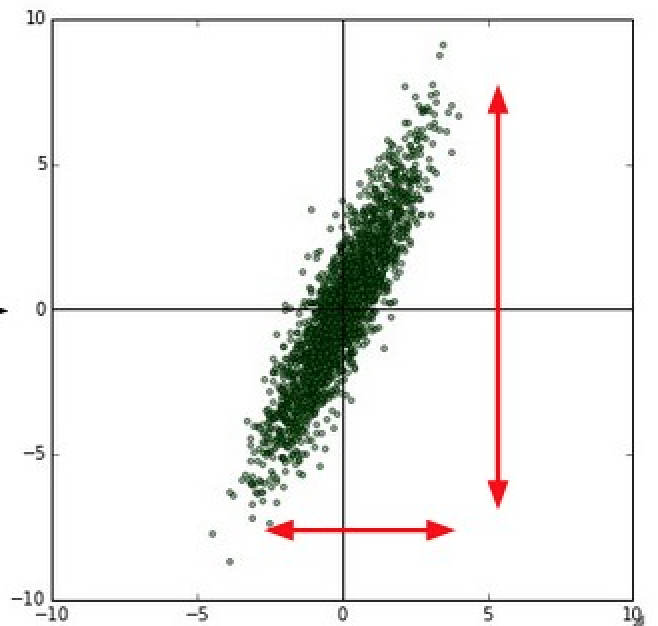
\includegraphics[width=200]{zero-centered.png}
\end{center}

Se observ\u{a} faptul c\u{a}, centrul datelor s-a mutat la origine.

Normalizarea datelor, presupune c\u{a} fiecare valoare din setul de date s\u{a} aibe aceea\c{s}i scal\u{a}, modul de a efectua acest lucru este de a \^{i}mp\u{a}r\c{t}i fiecare valoare din setul de date cu devia\c{t}ia standard pe care o are setul de date. Dac\u{a} vom aplica aceast\u{a} opera\c{t}ie pe setul de date vom ob\c{t}ine urmatorul grafic.

\begin{center}
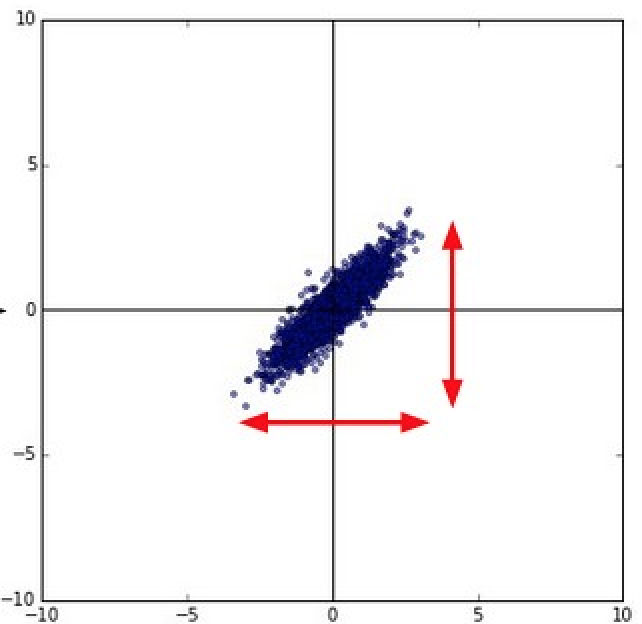
\includegraphics[width=200]{normalization.png}
\end{center}